\part{Complex-Eigen-Values}
\lecture{Complex Eigenvalues}{Complex-Eigen-Values}
\section{Complex Eigenvalues}


\title{Ordinary Differential Equations}
\subtitle{Math 232 - Week 11, Day 1}
\date{5 November 2012}

\begin{frame}
  \titlepage
\end{frame}

\begin{frame}
  \frametitle{Outline}
  \tableofcontents[pausesection,hideothersubsections]
\end{frame}


\subsection{Complex Valued Eigenvalues}


\begin{frame}
  \frametitle{Complex Valued Eigenvalues}

  First, recall:
  \begin{eqnarray*}
    e^{a+bi} & = & e^a e^{bi}, \\
    & = & e^a \lp \cos(b) + i \sin(b) \rp.
  \end{eqnarray*}

  Also, the complex conjugate:
  \begin{eqnarray*}
    \overline{a+ib} & = & a-i b.
  \end{eqnarray*}

  Note: If A is a real valued matrix with complex valued eigenvalues,
  then the eigenvalues and eigenvectors come in complex conjugates
  pairs.

\end{frame}

\iftoggle{clicker}{%
\begin{frame}
  \frametitle{Clicker Quiz}

   \ifnum\value{clickerQuiz}=1{%
     Express $\frac{1}{3-i}$ in rectangular form: \\ [12pt]
     \begin{tabular}{ll}
       A: & $\frac{1}{3} - i$ \\ [12pt]
       B: & $\frac{3}{10} + \frac{1}{10} i$ \\ [12pt]
       C: & $\frac{3}{10} - \frac{1}{10} i$ 
     \end{tabular}

     \vfill
   }\fi

   \ifnum\value{clickerQuiz}=2{%
     Express $\frac{1}{3-i}$ in rectangular form: \\ [12pt]
     \begin{tabular}{ll}
       A: & $\frac{1}{3} - i$ \\ [12pt]
       B: & $\frac{3}{10} - \frac{1}{10} i$ \\ [12pt]
       C: & $\frac{3}{10} + \frac{1}{10} i$ 
     \end{tabular}


   \vfill
   }\fi

  \ifnum\value{clickerQuiz}=3{%
   Given $A=\arrayTwo{-8}{30}{-3}{10}$. Find the eigenvalues.
   \begin{tabular}{ll}
     A: & $\lambda_{1,2} = 1 \pm 3i.$ \\
     B: & $\lambda_{1} = 4, \lambda_2 = -2.$ \\
     C: & $\lambda_{1,2} = 1.$ \\
   \end{tabular}

  \vfill
 }\fi
\end{frame}
}


\begin{frame}
  \frametitle{Example}

  \begin{eqnarray*}
    \deriv{~}{t} \vec{x} & = & \arrayTwo{-8}{30}{-3}{10} \vec{x}.
  \end{eqnarray*}

  \uncover<2->
  {
    Find the eigenvalues:
    \begin{eqnarray*}
      \det\lp\arrayTwo{-8-\lambda}{30}{-3}{10-\lambda}\rp 
      & = & \lambda^2-2\lambda+10 \\
      \lambda_{1,2} & = & 1 \pm 3i.
    \end{eqnarray*}
  }

\end{frame}


\begin{frame}
  \frametitle{Find the Eigenvectors}

  $\lambda_1 = 1+3i$:
  \begin{eqnarray*}
    \arrayTwo{-9-3i}{30}{-3}{9-3i} \vecTwo{x}{y} & = & \vecTwo{0}{0} \\
    x & = & \lp 3 - i \rp y, \\
    \Rightarrow \vec{v}_1 & = & y \lp \vecTwo{3}{1} + \vecTwo{-i}{0} \rp.
  \end{eqnarray*}

  \uncover<2->
  {
    $\lambda_2 = 1-3i$:
    \begin{eqnarray*}
      \arrayTwo{-9+3i}{30}{-3}{9+3i} \vecTwo{x}{y} & = & \vecTwo{0}{0} \\
      x & = & \lp 3+i \rp y, \\
      \Rightarrow \vec{v}_2 & = & y \lp \vecTwo{3}{1} - \vecTwo{-i}{0} \rp.
    \end{eqnarray*}
  }

\end{frame}


\begin{frame}
  \frametitle{Determine the Solution}

  \begin{eqnarray*}
    \uncover<1->
    {
      \vec{x} & = & A e^{(1+3i)t} \lp \vecTwo{3}{1} + \vecTwo{-i}{0} \rp
      + B e^{(1-3i)t} \lp \vecTwo{3}{1} - \vecTwo{-i}{0} \rp \\
    }
    \uncover<2->
    {
      \vec{x} & = & A e^{(1+3i)t} \lp \underbrace{\vecTwo{3}{1}}_{\vec{p}} + 
      \underbrace{\vecTwo{-i}{0}}_{i\vec{q}} \rp
      + B e^{(1-3i)t} \lp \underbrace{\vecTwo{3}{1}}_{\vec{p}} -
      \underbrace{\vecTwo{-i}{0}}_{i\vec{q}} \rp \\
    }
    \uncover<3->
    {
      & = & e^{t} \lp
        A \lp \cos(3t) + i \sin(3t) \rp \lp \vec{p} + i \vec{q} \rp + \right. \\
        & & \left. ~~~~
        B \lp \cos(3t) - i \sin(3t) \rp \lp \vec{p} - i \vec{q} \rp 
      \rp
    }
  \end{eqnarray*}

\end{frame}


\begin{frame}
  \frametitle{More Algebra...}

  \begin{eqnarray*}
    \vec{x} & = & e^{t} \lp
      A\lp \cos(3t) + i \sin(3t) \rp \lp \vec{p} + i \vec{q} \rp  \right. + \\
    & & \left.
  ~~~~ B \lp \cos(3t) - i \sin(3t) \rp \lp \vec{p} - i \vec{q} \rp \rp \\
  & = & C_1 e^{t} \lp \cos(3t) \vec{p} - \sin(3t) \vec{q} \rp
  + C_2 e^{t} \lp \cos(3t) \vec{q} + \sin(3t) \vec{p} \rp.
  \end{eqnarray*}

  (The solutions spiral out clockwise.)

  \only<2>{\centerline{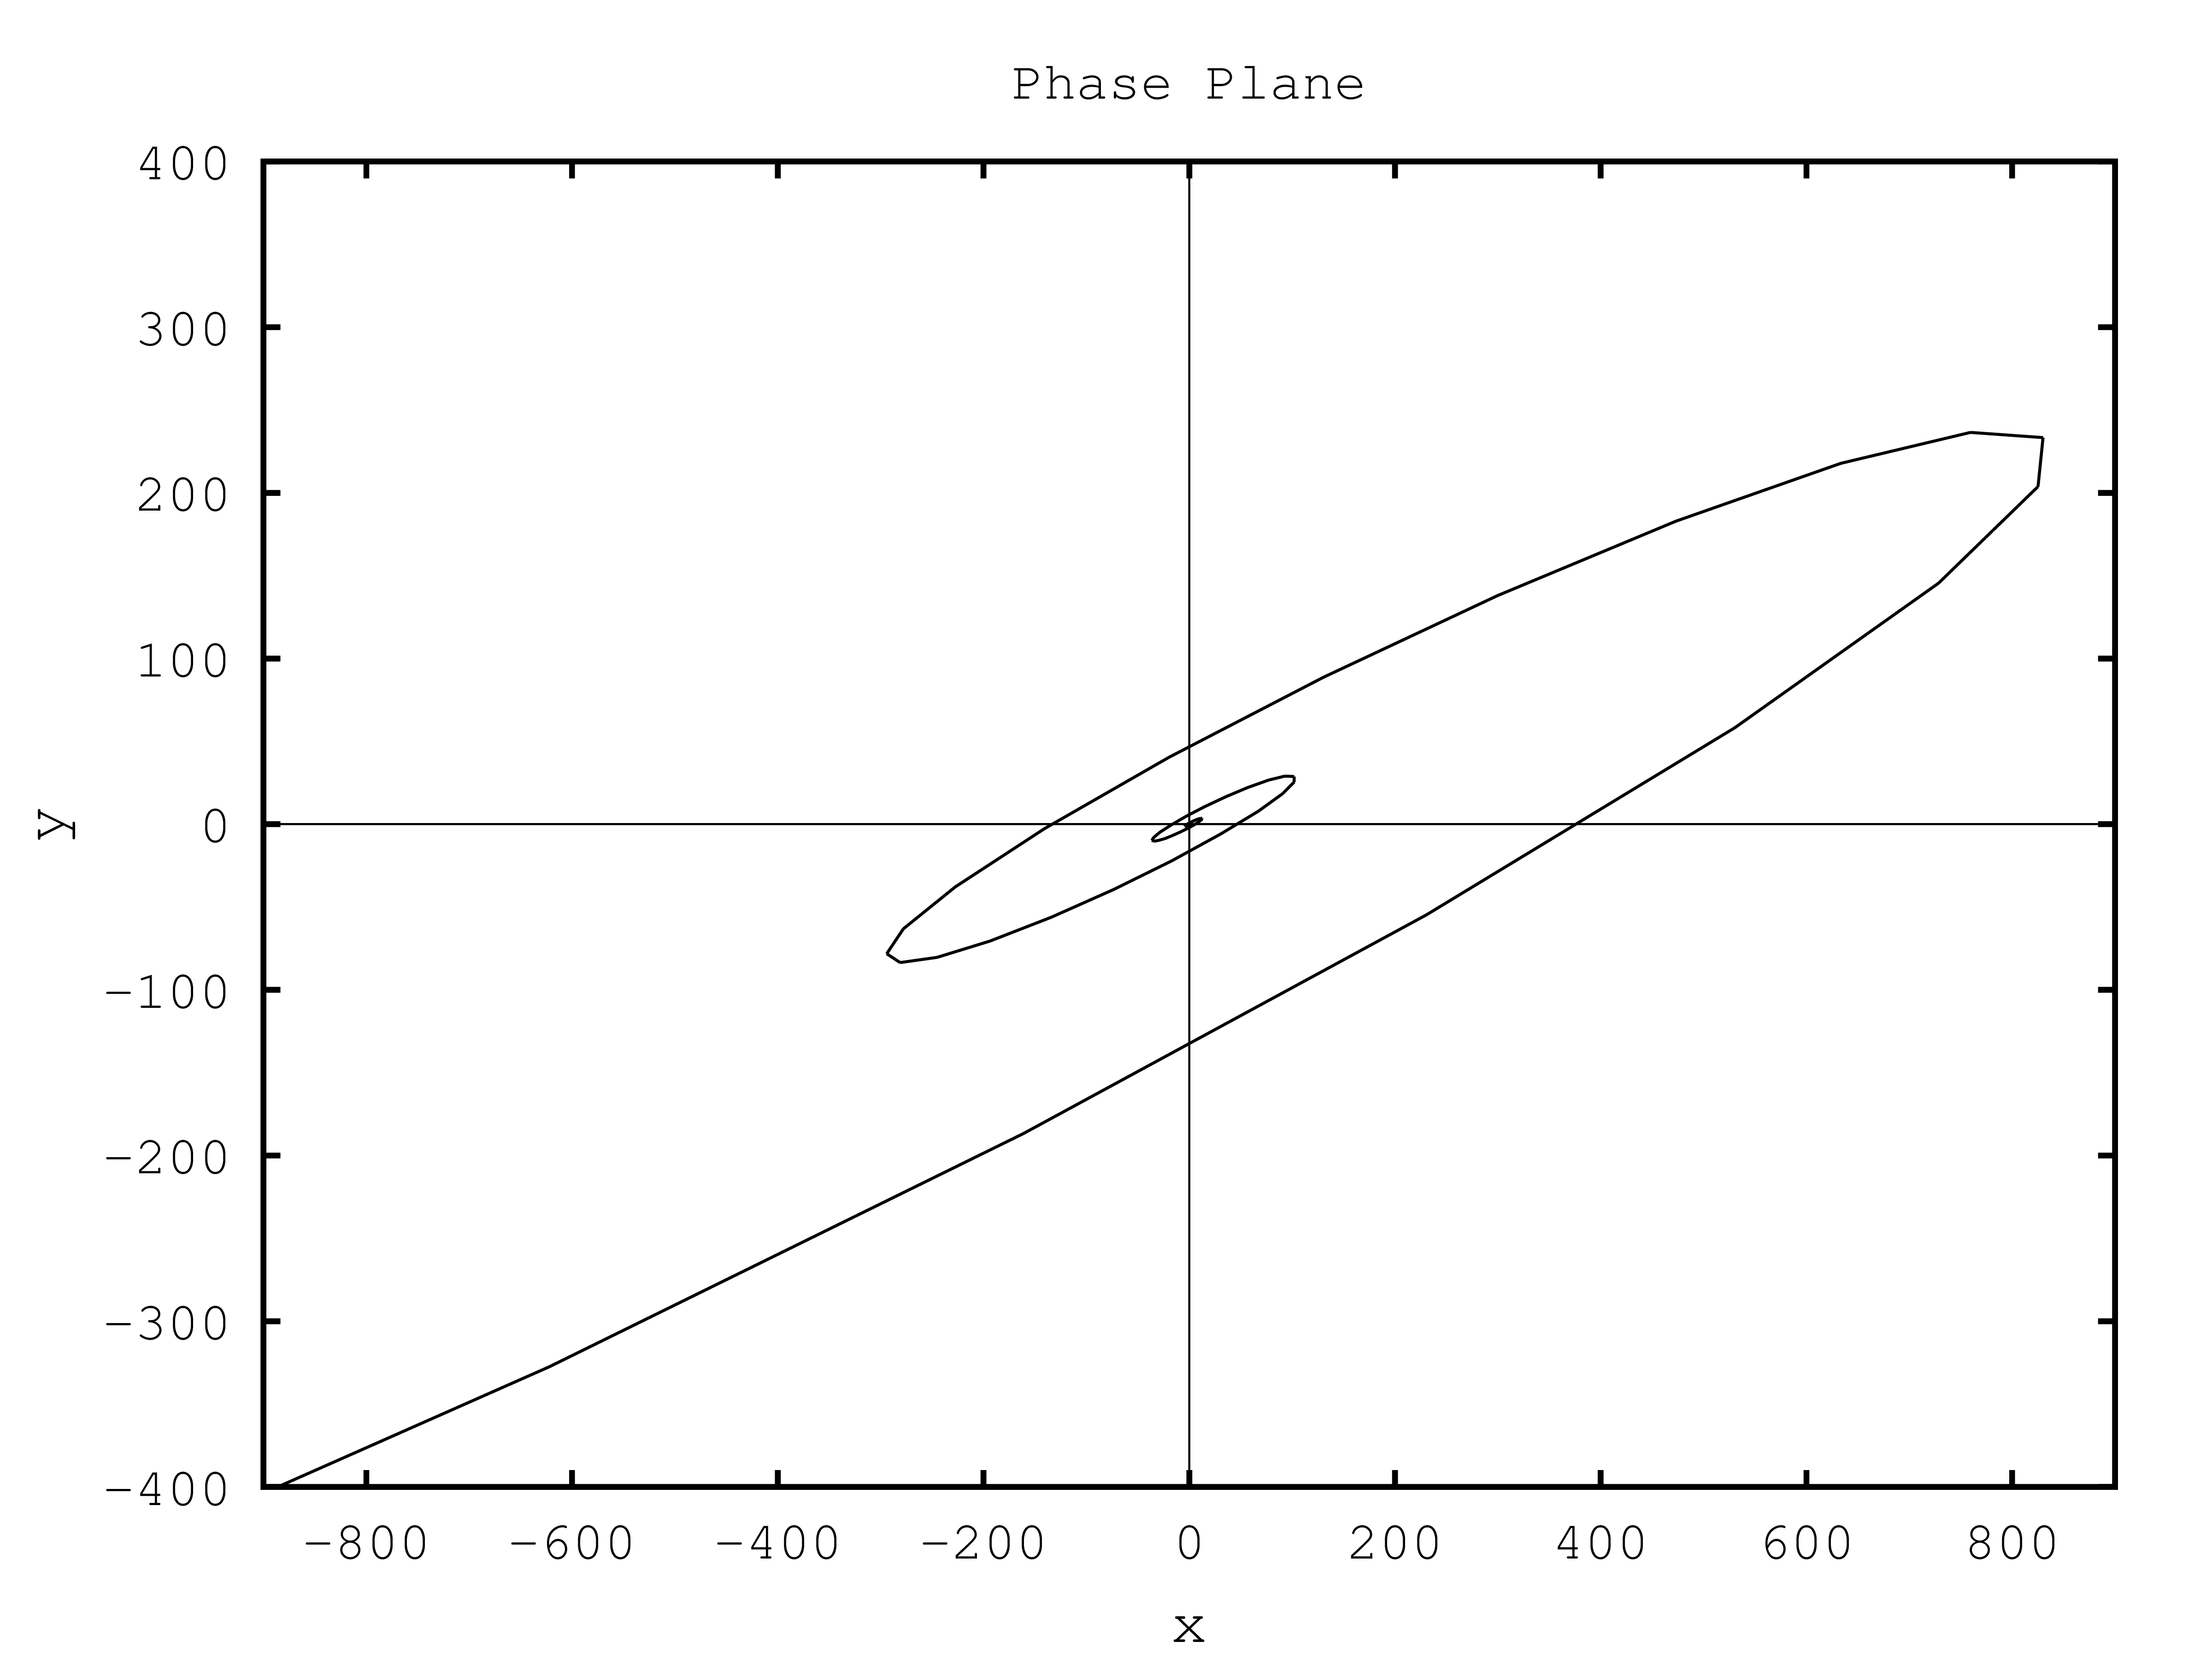
\includegraphics[width=4.5cm]{img/complexPhaseOne}}}
  \only<3>{\centerline{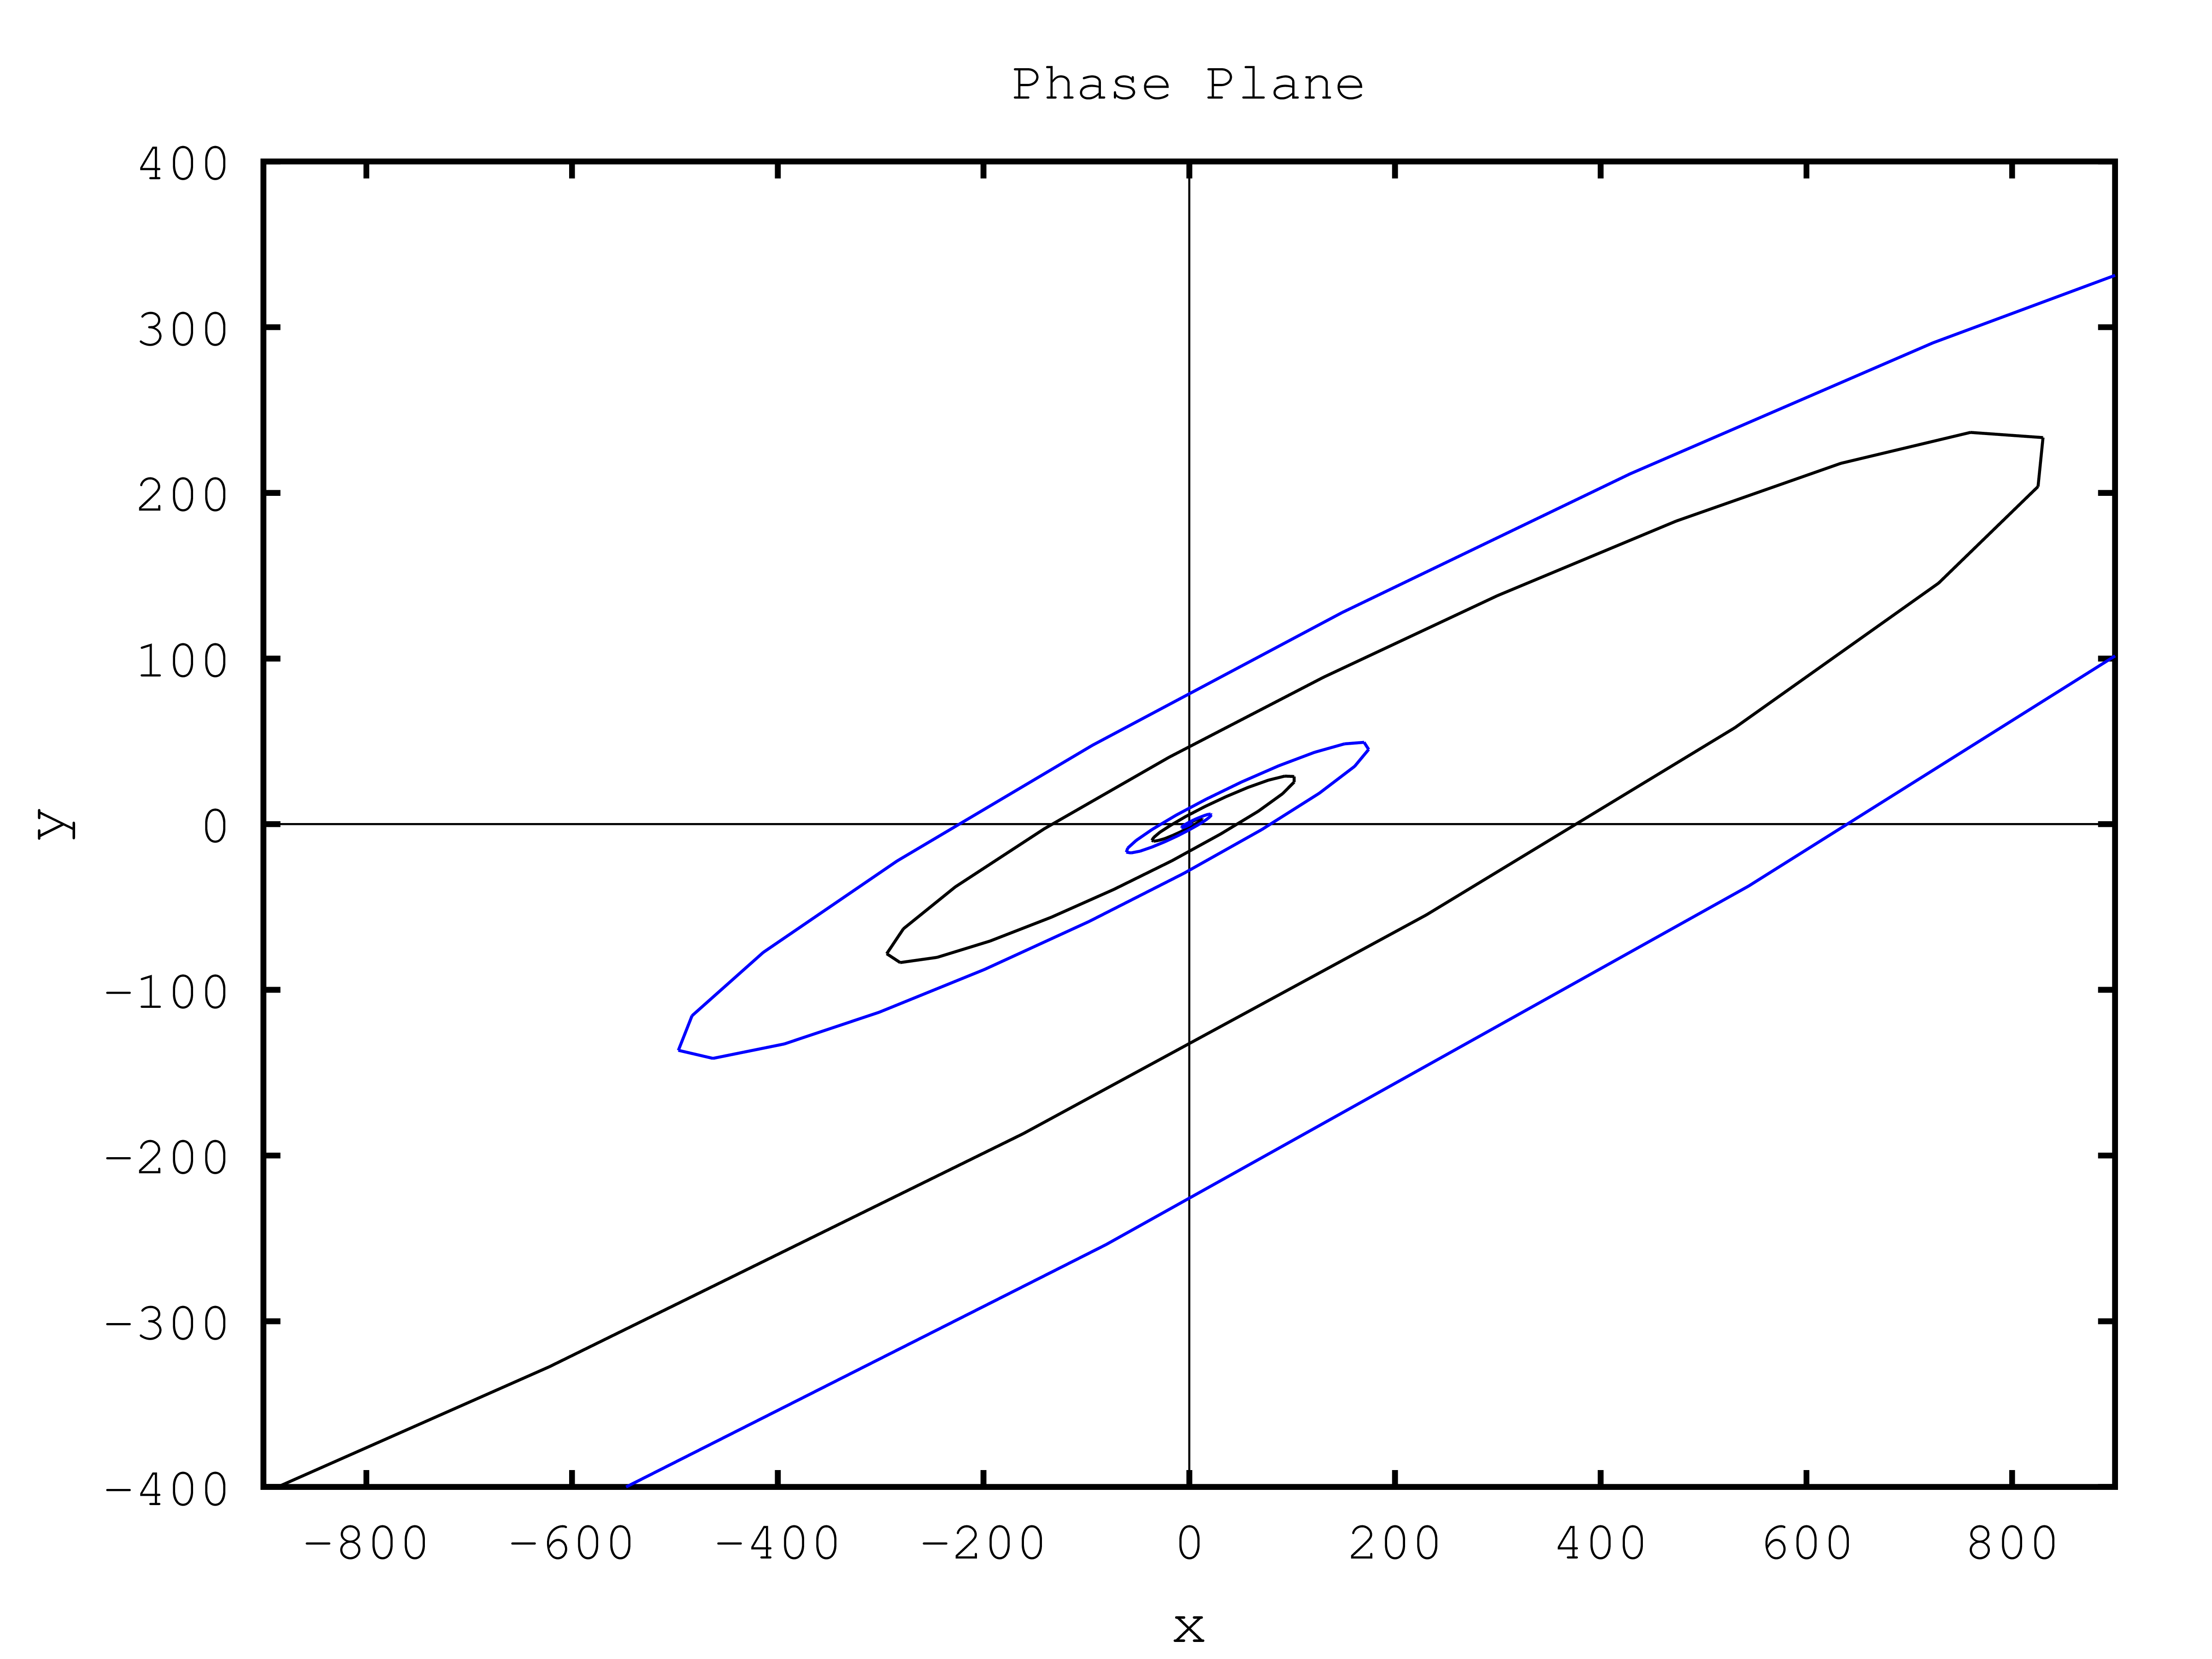
\includegraphics[width=4.5cm]{img/complexPhaseTwo}}}
  \only<4>{\centerline{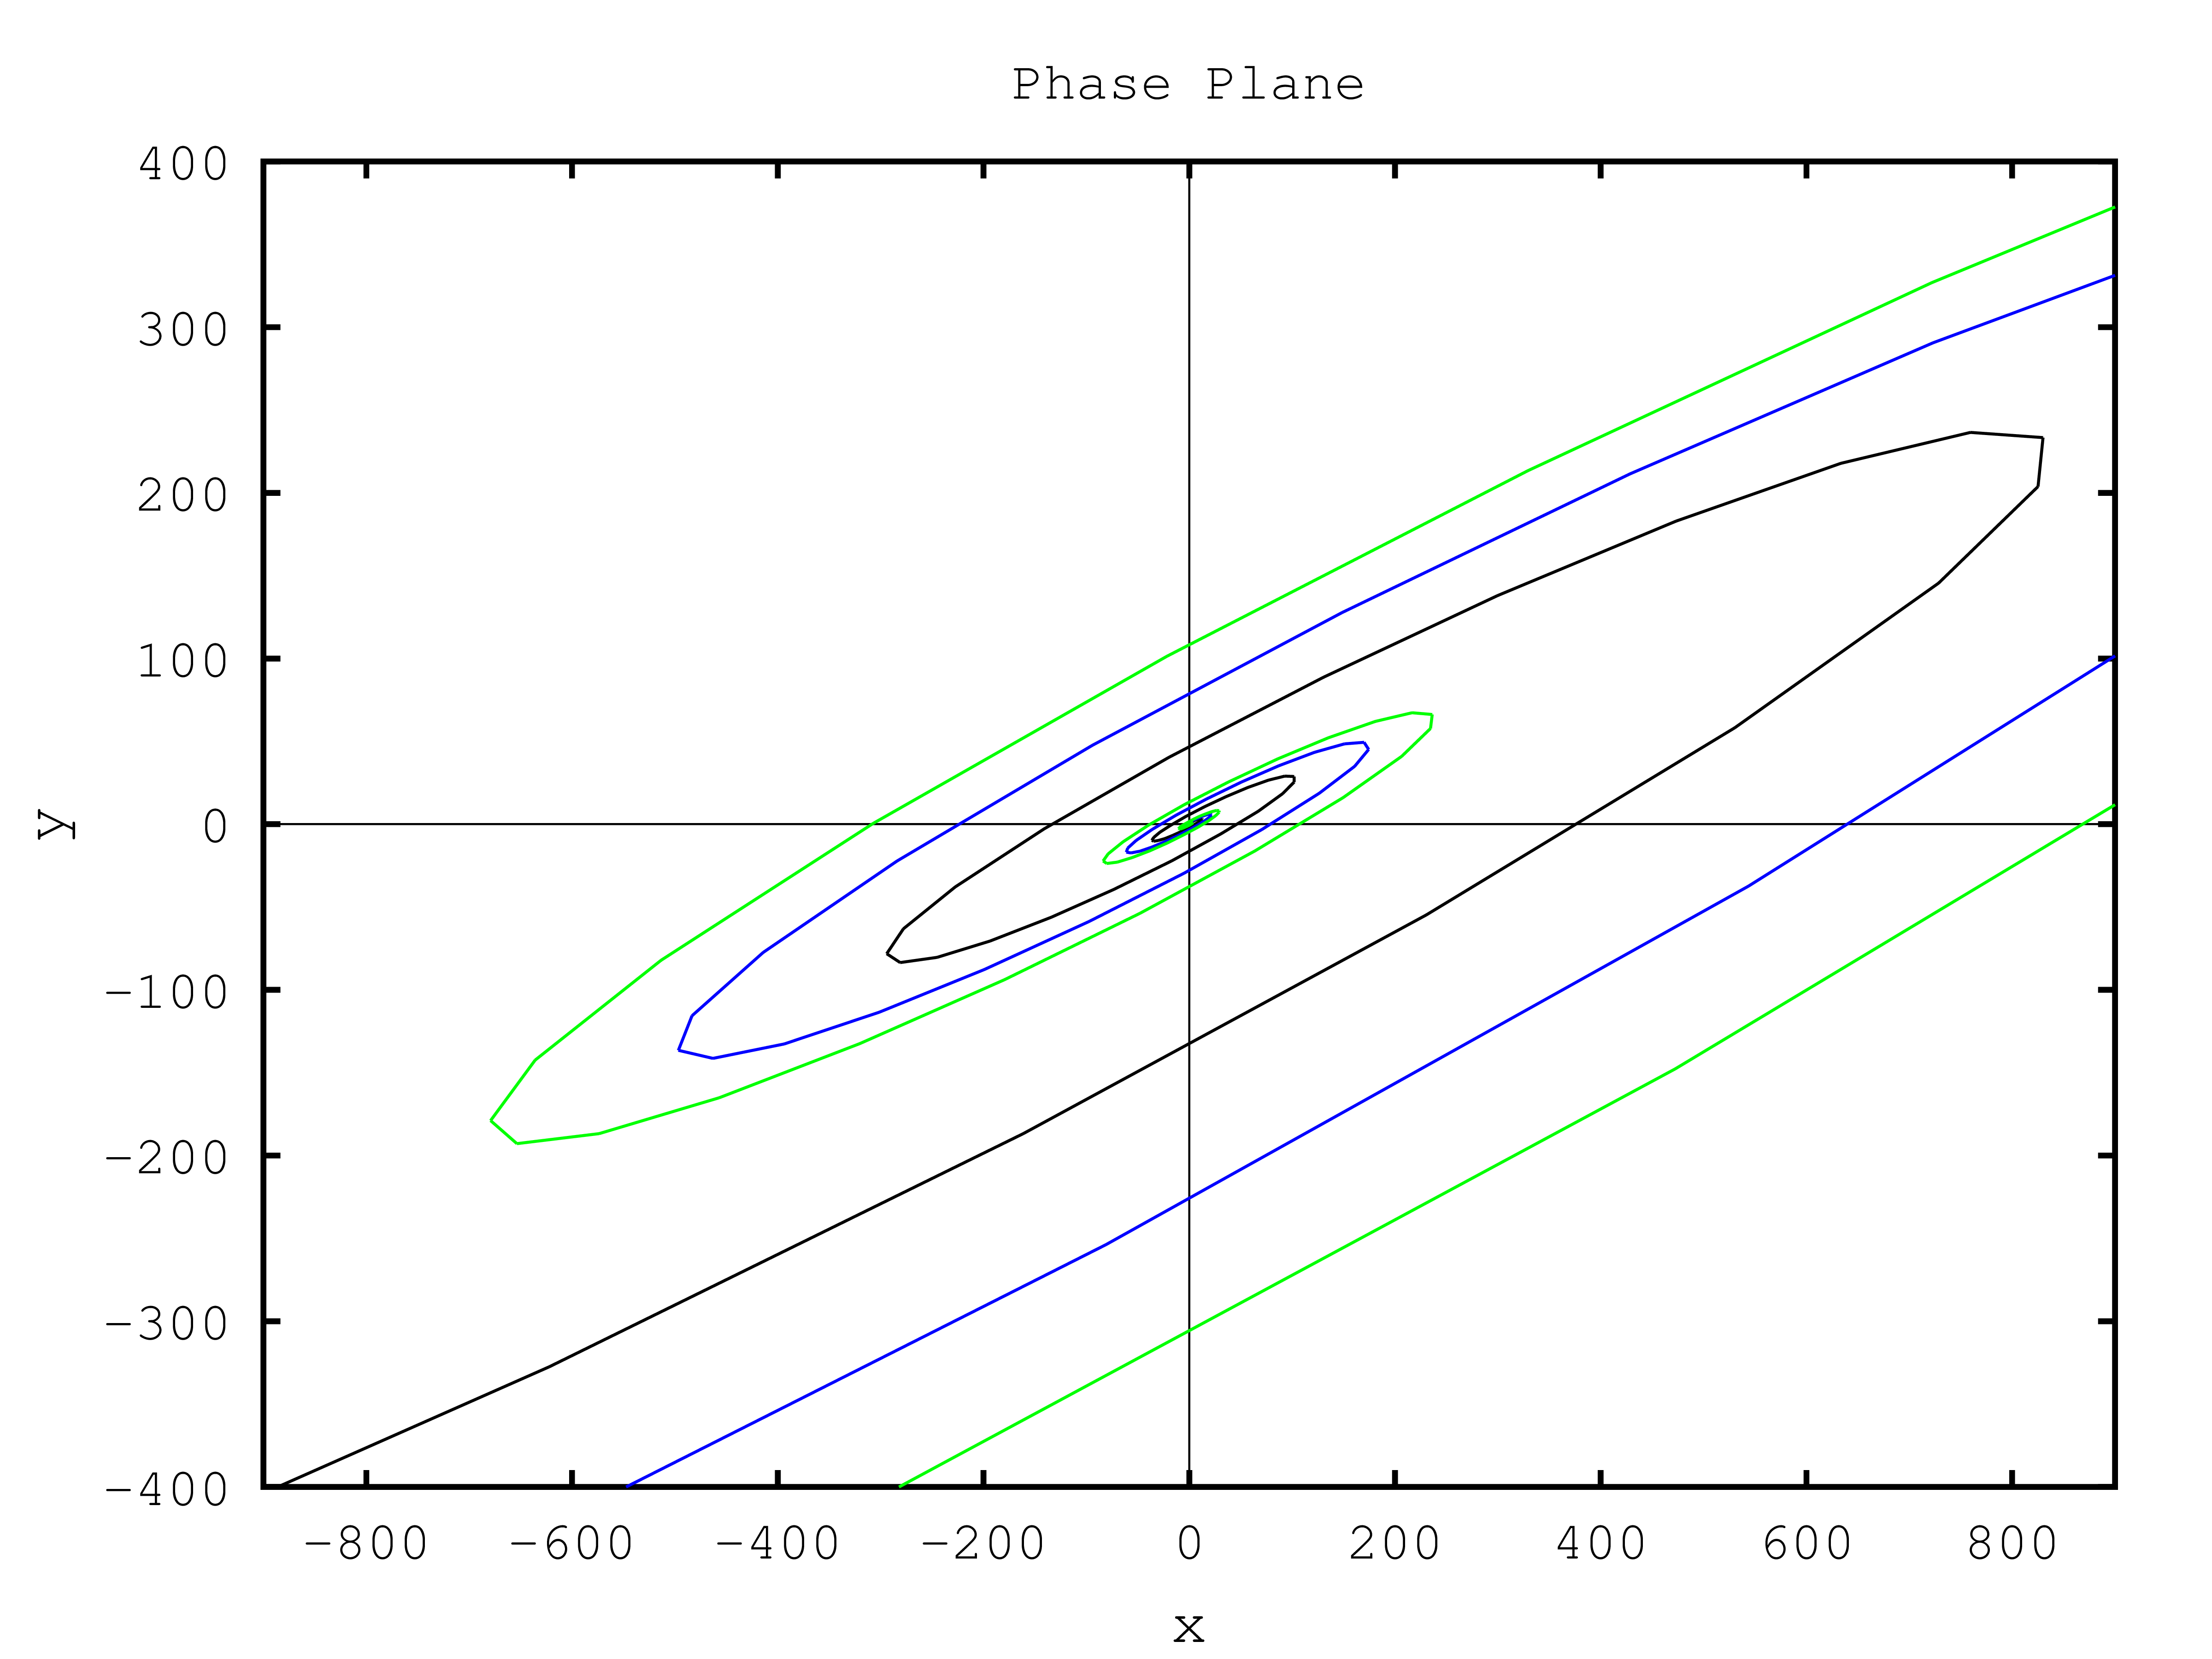
\includegraphics[width=4.5cm]{img/complexPhaseThree}}}

\end{frame}



\subsection{Characterization of Solutions}

\begin{frame}
  \frametitle{Characterization of Solutions}

  \begin{eqnarray*}
    \deriv{~}{t} \vec{x} & = & A \vec{x}.
  \end{eqnarray*}

  If $\lambda$'s are complex, $\lambda = a \pm ib$:
  \begin{enumerate}
  \item If $a>0$ then it is a repelling spiral (spiral source).
  \item If $a<0$ then it is an attracting spiral (spiral sink).
  \item If $a=0$ then the solutions are neutrally stable.
  \end{enumerate}

\end{frame}


\subsection{Nullclines}

\begin{frame}
  \frametitle{Nullclines}

  Given a solution to a differential equation,
  \begin{eqnarray*}
    \vec{x} & = & \vecTwo{x(t)}{y(t)},
  \end{eqnarray*}
  if
  \begin{itemize}
  \item $x'(t)=0$ then the trajectory is ``vertical'' at time $t$,
  \item $y'(t)=0$ then the trajectory is ``horizontal'' at time $t$.
  \end{itemize}

\end{frame}


\begin{frame}
  \frametitle{Definition of the Nullclines}

  The set of points, $\vecTwo{x}{y}$ where $x'(t)=0$ is called the v-nullcline. (Vertical slope.)

  The set of points, $\vecTwo{x}{y}$ where $y'(t)=0$ is called the h-nullcline. (Horizontal slope.)

\end{frame}


\begin{frame}
  \frametitle{Example}
  
  In the previous example we had
  \begin{eqnarray*}
    \deriv{~}{t} \vec{x} & = & \arrayTwo{-8}{30}{-3}{10} \vec{x}.
  \end{eqnarray*}

  \uncover<2->
  {
    Find the v-nullcline:
    \begin{eqnarray*}
      \deriv{x}{t} & = & -8x + 30y, \\
      0 & = & -8x + 30y, \\
      y & = & \frac{8}{30} x.
    \end{eqnarray*}
  }

  \uncover<3->
  {
    Find the h-nullcline:
    \begin{eqnarray*}
      \deriv{y}{t} & = & -3x + 10y, \\
      0 & = & -3x + 10y, \\
      y & = &  \frac{3}{10} x.
    \end{eqnarray*}
  }


\end{frame}


\begin{frame}
  \frametitle{Example - Graphical View}

  \centerline{\includegraphics[height=8.0cm]{img/complexPhaseNullClines}}  

\end{frame}

\begin{frame}
  \frametitle{Extra Example}

  Determine the solution to the system of equations given by
  \begin{eqnarray*}
    \deriv{~}{t} \vec{x} & = & \arrayTwo{1}{1}{-2}{3} \vec{x}.
  \end{eqnarray*}

  \uncover<2->
  {
    Find the eigenvalues:
    \begin{eqnarray*}
      \det\lp\arrayTwo{1-\lambda}{1}{-2}{3-\lambda}\rp 
      & = & \lambda^2-4\lambda+5 \\
      \lambda_{1,2} & = & 2 \pm i.
    \end{eqnarray*}
  }

\end{frame}

\begin{frame}
  \frametitle{Find the Eigenvectors}

  $\lambda_1 = 2+i$:
  \begin{eqnarray*}
    \arrayTwo{-1-i}{1}{-2}{1-i} \vecTwo{x}{y} & = & \vecTwo{0}{0} \\
    y & = & \lp 1+i \rp x, \\
    \Rightarrow \vec{v}_1 & = & x \lp \vecTwo{1}{1} + i \vecTwo{0}{1} \rp.
  \end{eqnarray*}

  \uncover<2->
  {
    $\lambda_2 = 2-i$:
    \begin{eqnarray*}
      \arrayTwo{-1+i}{1}{-2}{1+i} \vecTwo{x}{y} & = & \vecTwo{0}{0} \\
      y & = & \lp 1-i \rp x, \\
      \Rightarrow \vec{v}_2 & = & x \lp \vecTwo{1}{1} - i \vecTwo{0}{1} \rp.
    \end{eqnarray*}

  }

\end{frame}


\begin{frame}
  \frametitle{Determine the Solution}

  \begin{eqnarray*}
    \uncover<1->
    {
      \vec{x} & = & A e^{(2+i)t} \lp \underbrace{\vecTwo{1}{1}}_{\vec{p}} + i
      \underbrace{\vecTwo{0}{1}}_{\vec{q}} \rp
      + B e^{(2-i)t} \lp \underbrace{\vecTwo{1}{1}}_{\vec{p}} -
      i \underbrace{\vecTwo{0}{1}}_{\vec{q}} \rp \\[12pt]
    }
    \uncover<2->
    {
      & = & e^{2t} \lp
        A \lp  \cos(t) + i \sin(t) \rp \lp \vec{p} + i \vec{q} \rp 
          + 
        B \lp \cos(t) - i \sin(t) \rp \lp \vec{p} - i \vec{q} \rp 
      \rp\\[12pt]
    }
    \uncover<3->
    {
  & = & C_1 e^{2t} \lp \cos(t) \vec{p} - \sin(t) \vec{q} \rp
  +  C_2 e^{2t} \lp \cos(t) \vec{q} + \sin(t) \vec{p} \rp.
   }
  \end{eqnarray*}

  (The solutions spiral out clockwise.)


\end{frame}



% LocalWords:  Clarkson pausesection hideothersubsections Nullclines nullcline
